\chapter{Vorbereitung}

	\section{Theoretische Grundlagen}
	
    \subsection{Einteilung von Supraleitern}

	\subsection{BCS-Theorie}
Eine gute theoretische Beschreibung Supraleiter 1. Art bietet die BCS-Theorie. 
Zwar kann durch diese die Hochtemperatursupraleitung auch erklärt werden, das 
Prinzip der Paarbildung bleibt jedoch ungeklärt.

        \subsubsection{Cooper-Paare}
Grundlage der Supraleitung ist die Cooper-Paarbildung der Elektronen im Festkörper.
\vspace{3pt}\\
Es wird angenommen, dass ein Elektron, aufgrund seiner negativen Ladung, eine 
Deformationsspur hinterlässt. 
\begin{figure}[h]
    \centering
    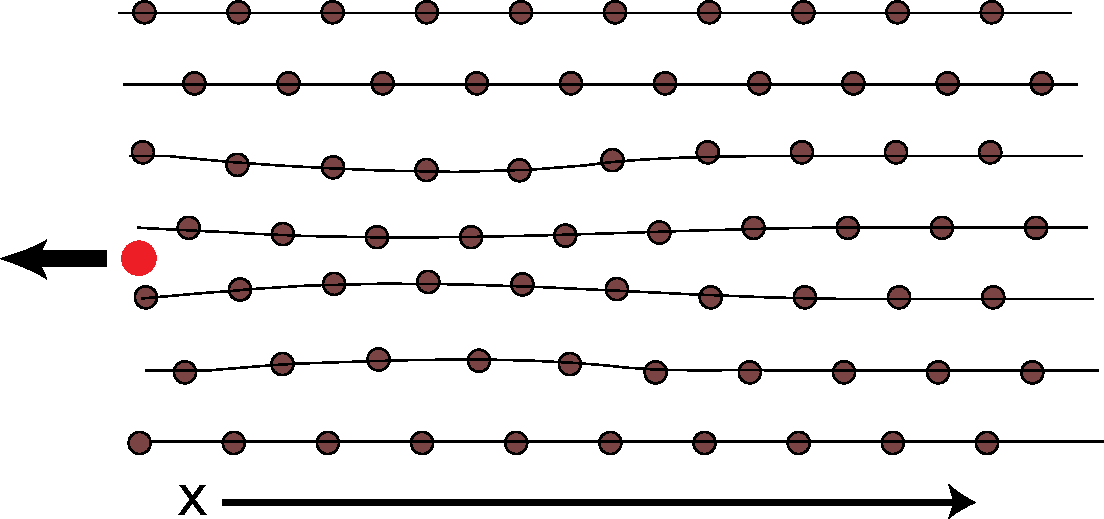
\includegraphics[width=0.7\textwidth]{Abb/deformation.pdf}
    \caption{Deformationsspur hinter einem Elektron}
    \label{Abb:def}
\end{figure}
Siehe hierzu Abbildung \ref{Abb:def}. Ein Elektron zieht die positiv geladenen Kerne
an, was diese zum Schwingen anregt. Nach einer viertel Schwingperiode erreicht die
Konzentration der positiven Ladungen ihr Maximum und weitere Elektronen werden 
angezogen. Durch die große Reichweite dieser Kraft, das erste Elektron ist nach
einer viertel Schwingperiode schon weit durch den Festkörper gewandert, wird sie
nicht durch die Coulomb-Abstoßung aufgehoben.
\vspace{3pt}\\
Grundlage der BCS-Theorie ist nun die Kopplung zweier Elektronen durch diese 
Wechselwirkung, wodurch der Verbund durch eine bosonische Gesamtwellenfunktion
beschrieben werden muss.

%\begin{itemize}
%    \item Bosonische Gesamtwellenfunktion
%    \item Stöße durch Energiezustand nicht möglich?
%    \item bosonen und fermionen
%\end{itemize}
